\documentclass{beamer}
\definecolor{links}{HTML}{2A1B81}

\usepackage[utf8]{inputenc}
\usepackage[norsk]{babel}
\usepackage{hyperref}
\hypersetup{
  colorlinks=true,
  linkcolor=,
  urlcolor=links
}

\usetheme{Copenhagen}
\usecolortheme{seahorse}

\definecolor{DMMH}{HTML}{F9F5EB}

\setbeamercolor{palette primary}{bg=DMMH,fg=black}
\setbeamercolor{palette secondary}{bg=DMMH,fg=black}
\setbeamercolor{palette tertiary}{bg=DMMH,fg=black}
\setbeamercolor{palette quaternary}{bg=DMMH,fg=black}

\title{Bibliotekorientering}
\author{Thomas Rambø\inst{1}}
\institute[DMMH-biblioteket]{
  \inst{1}
  Biblioteket\\
  Dronning Mauds Minne Høgskole
}

\date[DMMH 2018]{DMMH, høsten 2018}
\logo{
\includegraphics[height=1cm]{../media/logo.png}}

\AtBeginSection[]
{
  \begin{frame}
    \frametitle{Innhold}
    \tableofcontents[currentsection]
  \end{frame}
}

\begin{document}

\frame{\titlepage}
\begin{frame}
  \frametitle{Innhold}
  \tableofcontents
\end{frame}

\section{Velkommen til biblioteket}
\begin{frame}
  \frametitle{Velkommen til biblioteket}
  \centering
  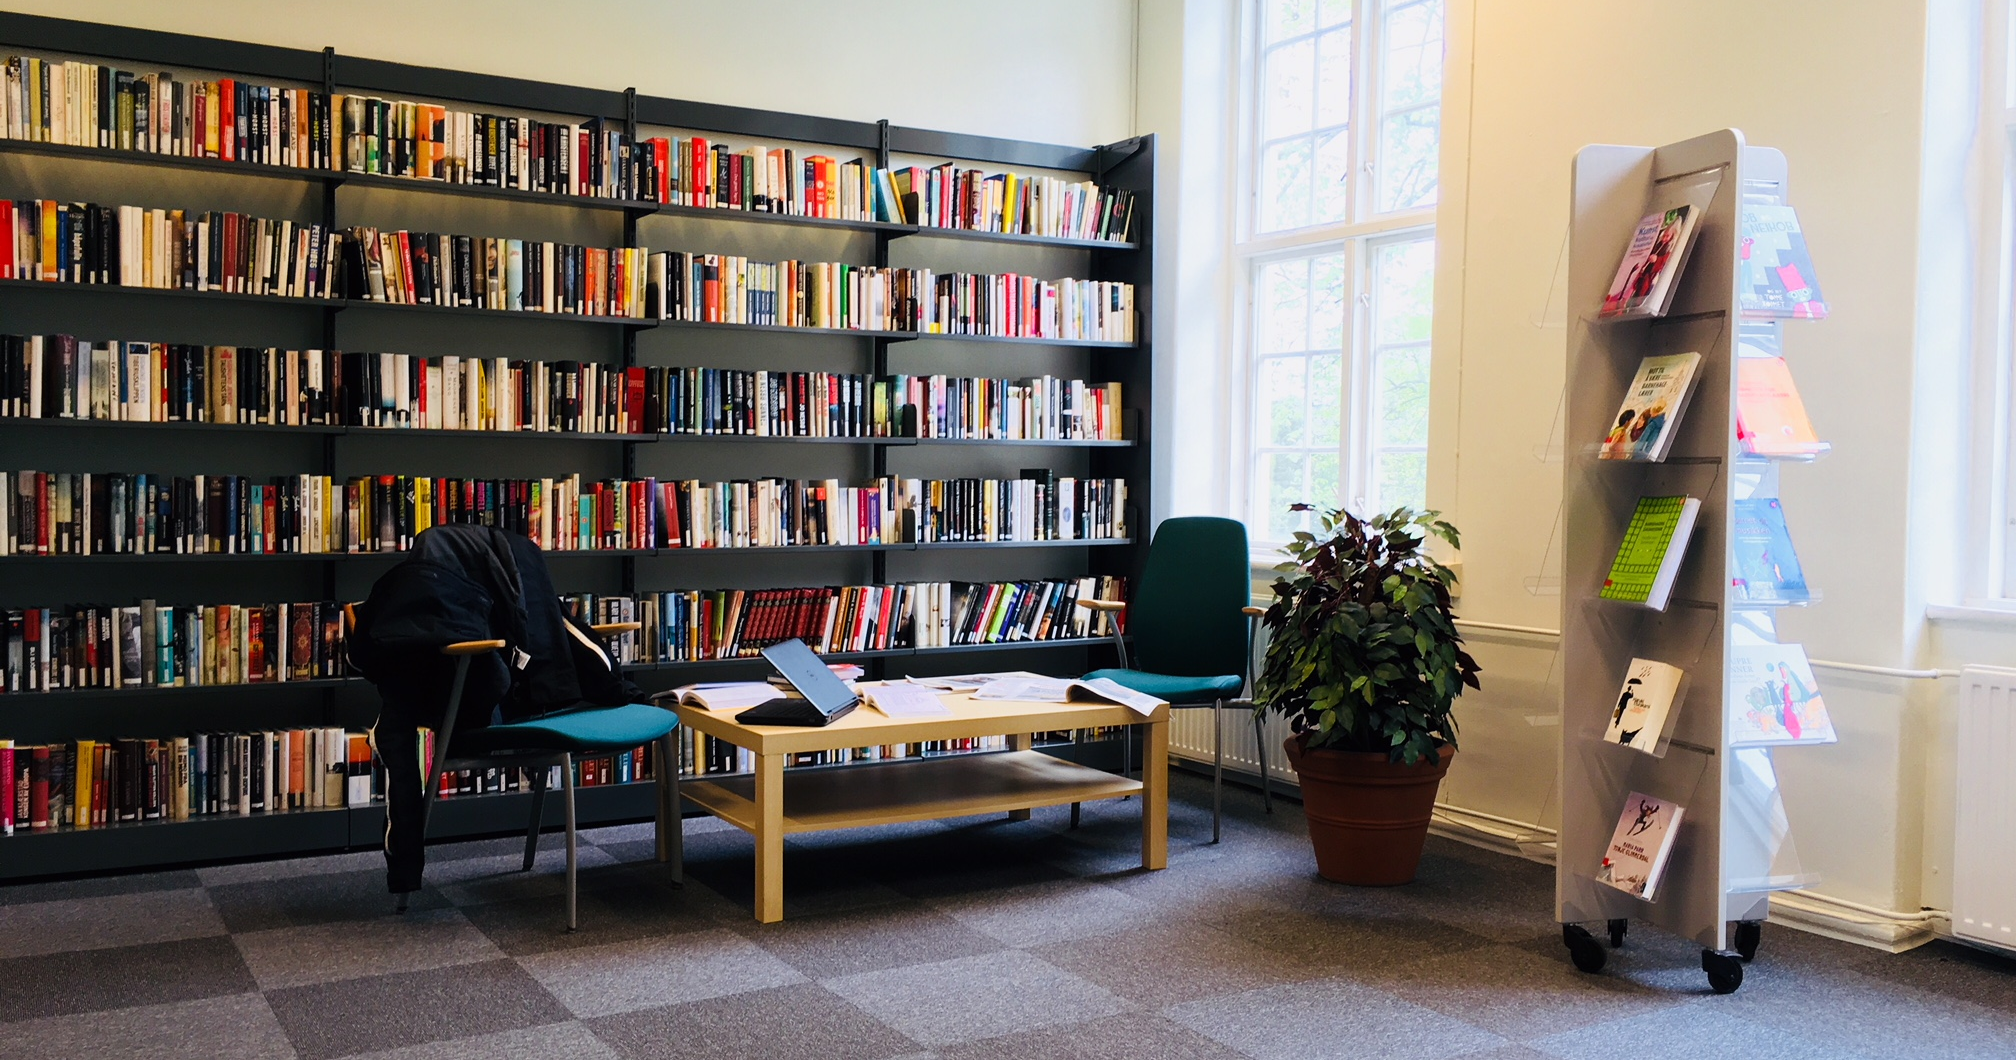
\includegraphics[width=0.90\textwidth]{../media/nytt-bibliotek.png}
\end{frame}
\begin{frame}
  Biblioteket ligger i 2. etasje i hovedbygget, og holder åpent mandag til fredag. Mandager og onsdager er åpningstidene \alert{08:30 til 19:00}, og ellers er åpningstidene \alert{08:30 til 15:30}.
\end{frame}
\begin{frame}
  \centering
  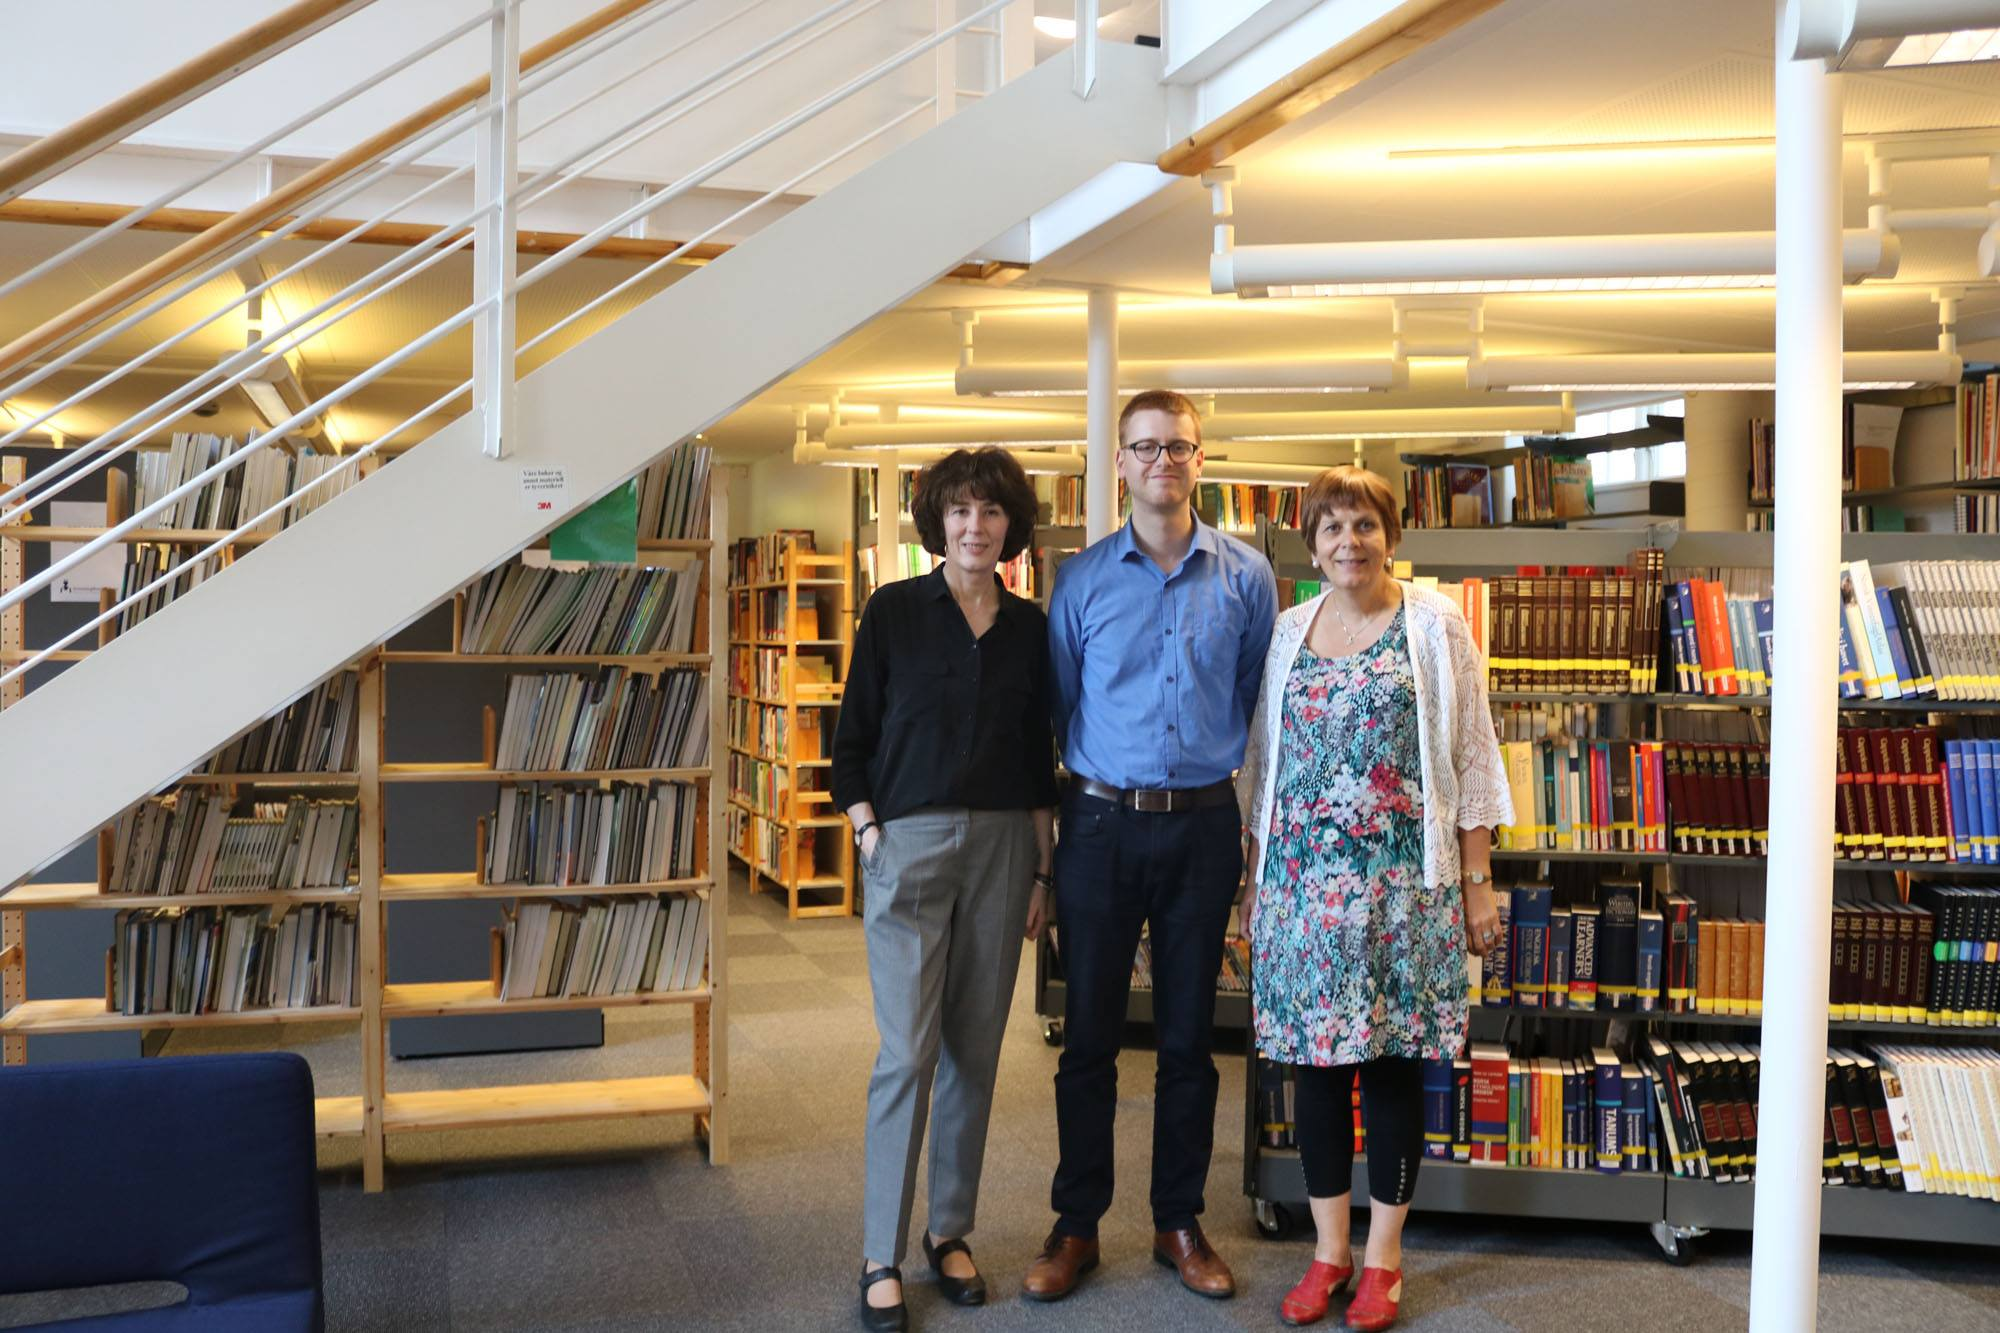
\includegraphics[width=0.90\textwidth]{../media/bibliotekansatte.jpg}
\end{frame}
\begin{frame}
  Personalet på biblioteket er på jobb for å bistå deg.

  \vfill
  \begin{tabular}{ l | l }
    Besøk oss: & Biblioteket ligger i 2. etasje i hovedbygget. \\
    På Facebook: & \url{https://m.me/dmmhbib} \\
    Telefon: & \texttt{73 80 52 42} \\
    E-post: & \href{mailto:bibliotek@dmmh.no}{bibliotek@dmmh.no}
  \end{tabular}
\end{frame}

\section{Hvilke tjenester kan biblioteket tilby?}
\subsection{Pensumlitteratur og annen støttelitteratur}
\begin{frame}
  \frametitle{Pensumlitteratur og annen støttelitteratur}
  Bibliotekets samling består blant annet av \alert{pensumlitteratur} og annen \alert{støttelitteratur}. Det er flere eksemplarer tilgjengelig, og som regel ett eksemplar av hver utgivelse som bare kan leses i bibliotekets lokaler.

  \vfill

  \begin{block}{Bemerkning}
    Bruk søketjenesten \href{http://bibsys-almaprimo.hosted.exlibrisgroup.com/primo_library/libweb/action/search.do?vid=DMMH}{Oria} til å finne fram litteraturen, og til å legge inn \href{https://dmmh.no/bibliotek/bestillinger}{bestillinger} på bøker som er lånt ut av andre. \textit{Nesten} alt finnes i Oria.
  \end{block}
\end{frame}

\subsection{Vitenskapelig arkiv}
\begin{frame}
  \frametitle{Vitenskapelig arkiv}
  \begin{columns}
    \column{0.5\textwidth}
    I den digitale samlingen har vi et \href{https://brage.bibsys.no/xmlui/handle/11250/92951}{vitenskapelig arkiv} med forskningsresultater fra DMMH og fremragende studentoppgaver på bachelor- og masternivå.

    \column{0.5\textwidth}
    \begin{figure}
      \caption{Forsiden av en bacheloroppgave i BIBSYS Brage.}
      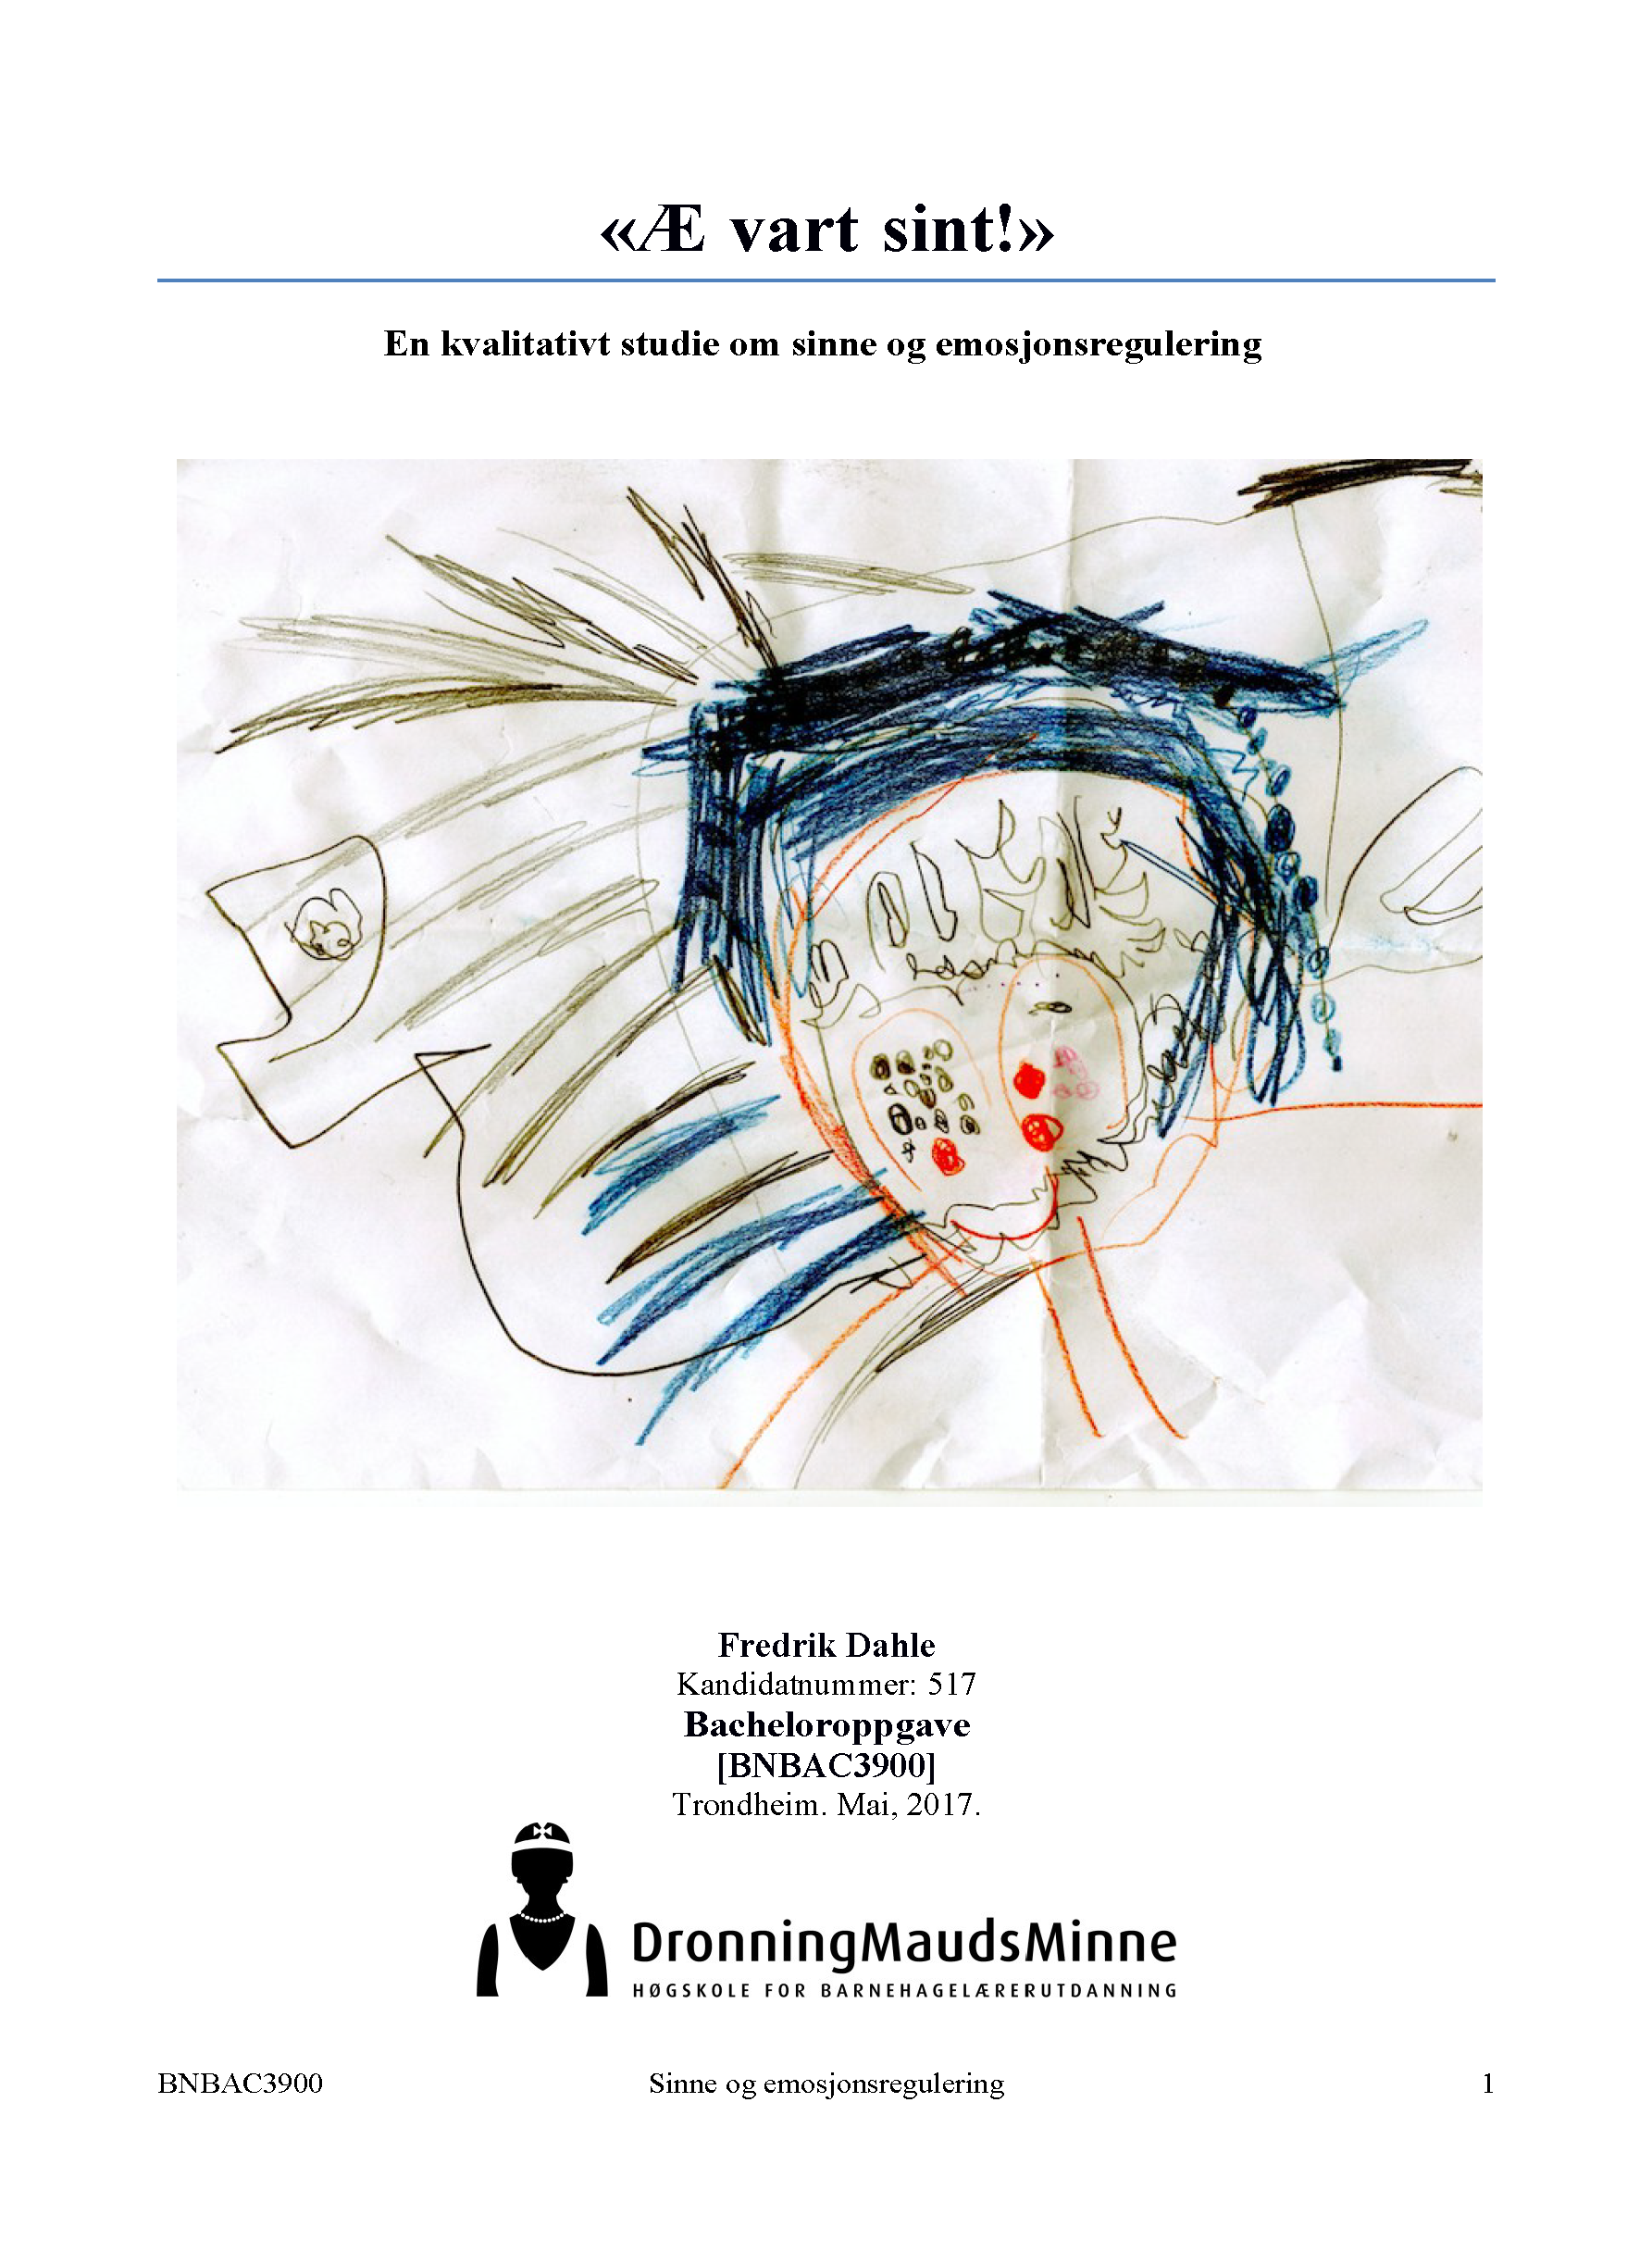
\includegraphics[width=0.6\textwidth]{../media/front-dahle.png}
    \end{figure}
  \end{columns}
\end{frame}

\subsection{Bibliografisk veiledning}
\begin{frame}
  \frametitle{Bibliografisk veiledning}
  På Dronning Maud brukes en spesifikk \alert{referansestil} på sitering og bibliografier i studentoppgaver. Denne er basert på APA 6. utgave, og biblioteket kan besvare spørsmål om riktig referering og bibliografisk utforming.

  \vfill

  \begin{block}{Bemerkning}
    Nettjenesten \href{https://sokogskriv.no/}{Søk \& Skriv} har nyttig informasjon om det å skrive oppgaver og hvordan man setter opp en referanseliste.
  \end{block}
\end{frame}
\begin{frame}
  \frametitle{Referansehåndteringsverktøyet Zotero}
  \begin{columns}
    \column{0.5\textwidth}
    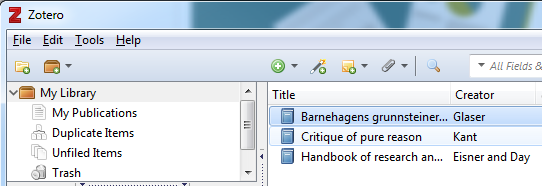
\includegraphics[width=1\textwidth]{../media/zotero.png}
    
    \column{0.5\textwidth}
    Referansehåndteringsverktøy kan strukturere og ordne referanselister og siteringer i oppgaver. \href{https://dmmh.no/bibliotek/skriving-og-referering/zotero}{Zotero} er gratis og kan automatisk opprette referanser fra innførsler i bibliotekkatalogen, litteraturdatabaser og ordinære nettsider. Zotero støtter norsk APA 6. utgave.
  \end{columns}
\end{frame}

\section{Bruke biblioteket}
\begin{frame}
  \frametitle{Bibliotekets nettsider}
  \begin{columns}
    \column{0.5\textwidth}
    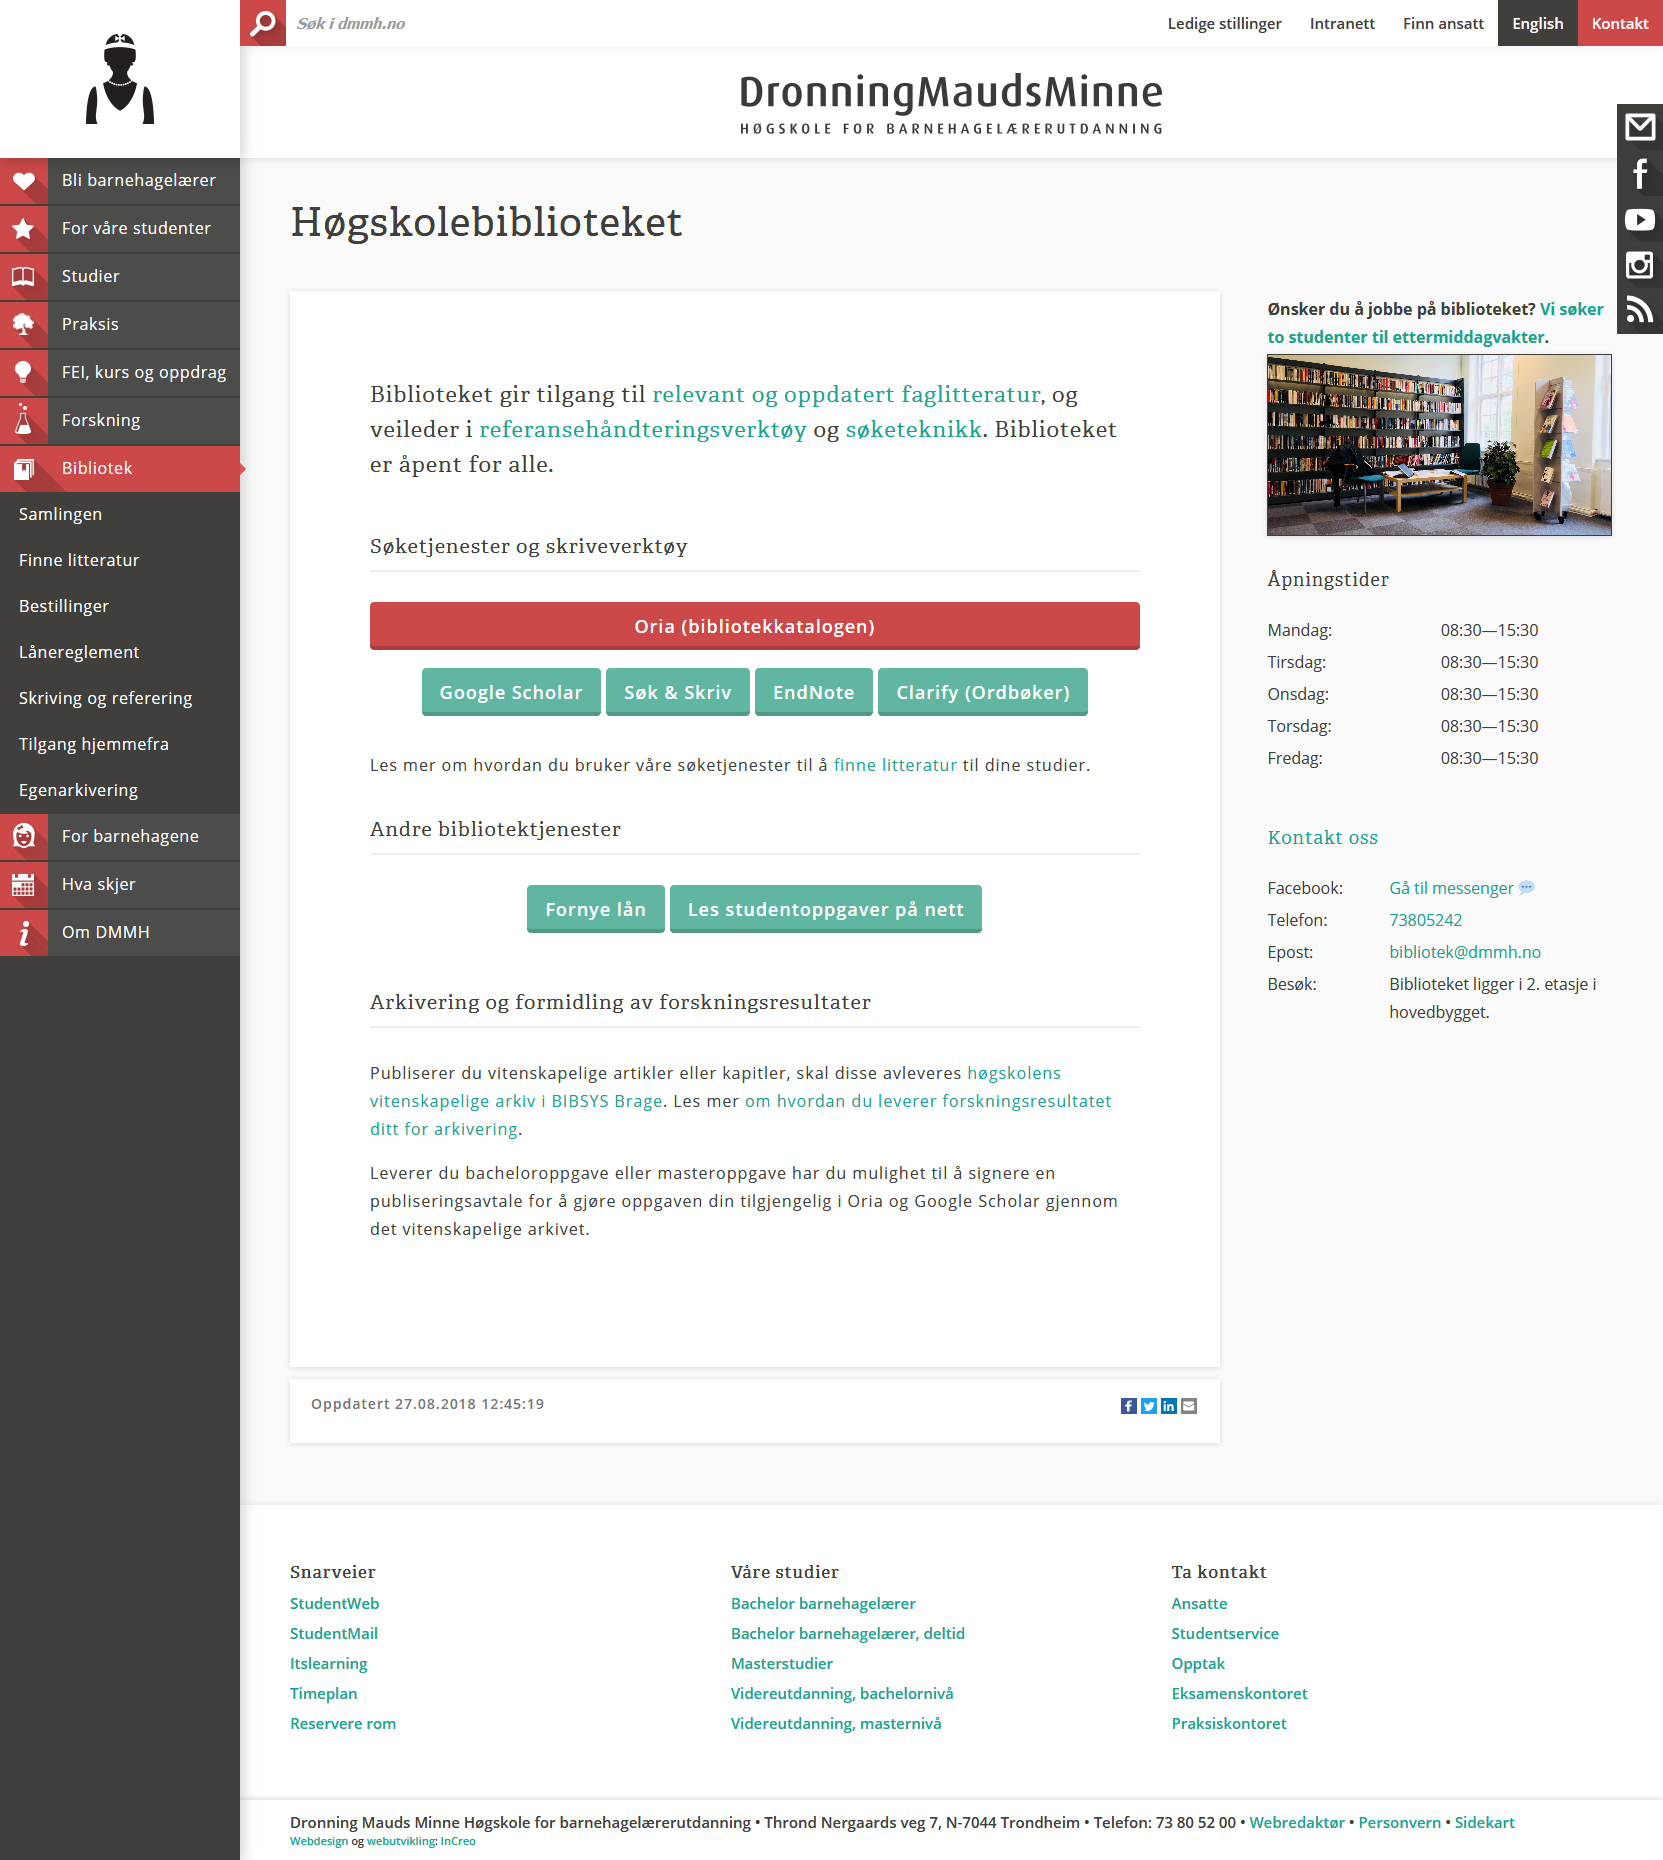
\includegraphics[width=0.8\textwidth]{../media/biblioteknettsiden.png}

    \column{0.5\textwidth}
    \begin{itemize}
    \item Bruk bibliotekets nettsider til å finne informasjon om hvordan du bruker biblioteket.
    \item Det er også hjelpesider med informasjon om søk og gjenfinning av litteratur, og bruk av referansehåndteringsverktøy.
    \end{itemize}
  \end{columns}
\end{frame}
\subsection{Lese og jobbe på biblioteket}
\begin{frame}
  \frametitle{Lese og jobbe på biblioteket}
  Det er sittegrupper i hoveddelen av biblioteket, arbeidsplasser og grupperom oppe på mesaninen og bord for gruppearbeid over gangen.
\end{frame}
\begin{frame}
  \frametitle{Litt å merke seg om jobbing på biblioteket}

  \begin{itemize}
  \item Ta hensyn til andre! Det er lov å snakke og samarbeide med andre, men hold lydnivå i hoveddelen av biblioteket på et lavt nivå.
  \item Mat og drikke er ikke tillatt inne på biblioteket, unntatt flaske eller kopp med lokk.
  \end{itemize}
\end{frame}
\subsection{Finne pensumlitteratur}
\begin{frame}
  \frametitle{Finne pensumlitteratur}
  Bruk \href{https://studier.dmmh.no}{studier.dmmh.no} til å finne pensumlister, og søk opp referanser i \href{http://bibsys-almaprimo.hosted.exlibrisgroup.com/primo_library/libweb/action/search.do?vid=DMMH}{Oria} for å finne plassering og evt. sette seg på venteliste.
\end{frame}

\subsection{Utlån, fornying og retur}
\begin{frame}
  \frametitle{Utlån og retur}

  \begin{columns}
    \column{0.5\textwidth}
    \centering
    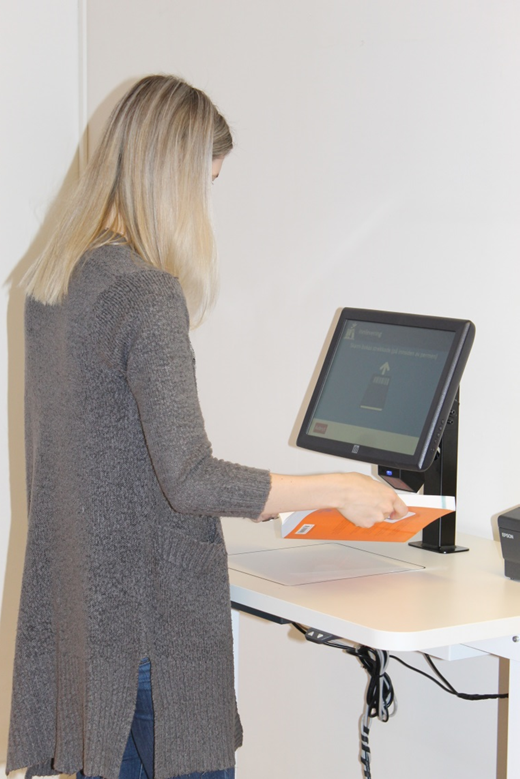
\includegraphics[width=0.8\textwidth]{../media/utlaansautomat.png}

    \column{0.5\textwidth}
    \begin{itemize}
    \item Du kan låne og returnere bøker selv ved å bruke selvbetjentautomaten som står i gangen. For å låne bøker trengs \alert{studentkortet}.
    \item Vi som står i skranken kan også registrere lån og retur for deg, for eksempel hvis du har glemt studentkortet eller trenger å fornye lån.
    \end{itemize}
  \end{columns}
\end{frame}

\begin{frame}
  \frametitle{Litt å merke seg om utlån}

  \begin{itemize}
  \item Studentkortet ditt fungerer som lånekort, men du kan også bruke \alert{Studentbevis-appen} på iOS og Android-telefoner. Hvis du får problemer med kortet kan du alltid kontakte oss i skranken.
  \item Alt materiale på biblioteket er utstyrt med \alert{alarm}, og alarmen kan bare deaktiveres når materialet blir registrert som lån på din konto.
  \item Materialet i pensumsamlingen er merket med rød tape og kan lånes ut i 2 uker. Øvrig materiale har vanligvis lånetid på 4 uker.
  \end{itemize}
\end{frame}

\begin{frame}
  \frametitle{Fornying av lån}

  \begin{itemize}
  \item På forfallsdato blir du automatisk kontaktet av biblioteksystemet, og du må levere materialet.
  \item Du kan når som helst \href{https://bibsys-almaprimo.hosted.exlibrisgroup.com/primo_library/libweb/action/login.do?loginFn=signin&vid=DMMH&targetURL=https://bibsys-almaprimo.hosted.exlibrisgroup.com/primo_library/libweb/action/myAccountMenu.do?vid=DMMH&fromLink=gotoMyAccountUI}{fornye lån i Oria}, forutsatt at ingen står på venteliste på materialet.
  \item Lån + fornying er satt til maksimalt 45 dager for pensum og 90 dager for øvrig materiale. Kontakt biblioteket for å låne materialet lengre.
  \end{itemize}
\end{frame}

\begin{frame}
  \frametitle{Reservering og bestilling}

  \begin{itemize}
  \item Bøker som er lånt ut kan reserveres av andre.
  \item Når boka blir tilgjengelig sendes en hentebeskjed til neste i køen.
  \item Bestillinger fra lager og fra andre bibliotek gjør også at hentebeskjed sendes.
  \end{itemize}
\end{frame}
\end{document}
